% =================================================================================================
% File:			registrazione_e_autenticazione.tex
% Description:	Definisce la sezione relativa ad un capitolo del documento
% Created:		2015-04-21
% Author:		Santacatterina Luca
% Email:		santacatterina.luca@mashup-unipd.it
% =================================================================================================
% Modification History:
% Version		Modifier Date		Change											Author
% 0.0.1 		2015-05-24 			inizio stesura sezione capitolo					Santacatterina Luca
% =================================================================================================
%

% CONTENUTO DEL CAPITOLO
\section{Configurazione utente} % (fold)
\label{sec:configurazione_utente}
	Dopo aver eseguito le istruzioni per l'autenticazione\gloss{} viene visualizzata la dashboard\gloss{} dell’applicazione.\newline
	Cliccando sull'icona del menù utente (Figura: \ref{fig:menu_configurazione_utente}, rif. 1) presente in alto a destra nella schermata principale si ottengono le seguenti opzioni:
	\begin{itemize}
		\item Settings (Figura: \ref{fig:menu_configurazione_utente}, rif. 2);
		\item API Token config (Figura: \ref{fig:menu_configurazione_utente}, rif. 3);
		\item Logout (Figura: \ref{fig:menu_configurazione_utente}, rif. 4).
	\end{itemize}
	Ogni voce del menù ricopre un ruolo di personalizzazione del profilo utente.
	\begin{figure}[H]
		\centering
		\centerline{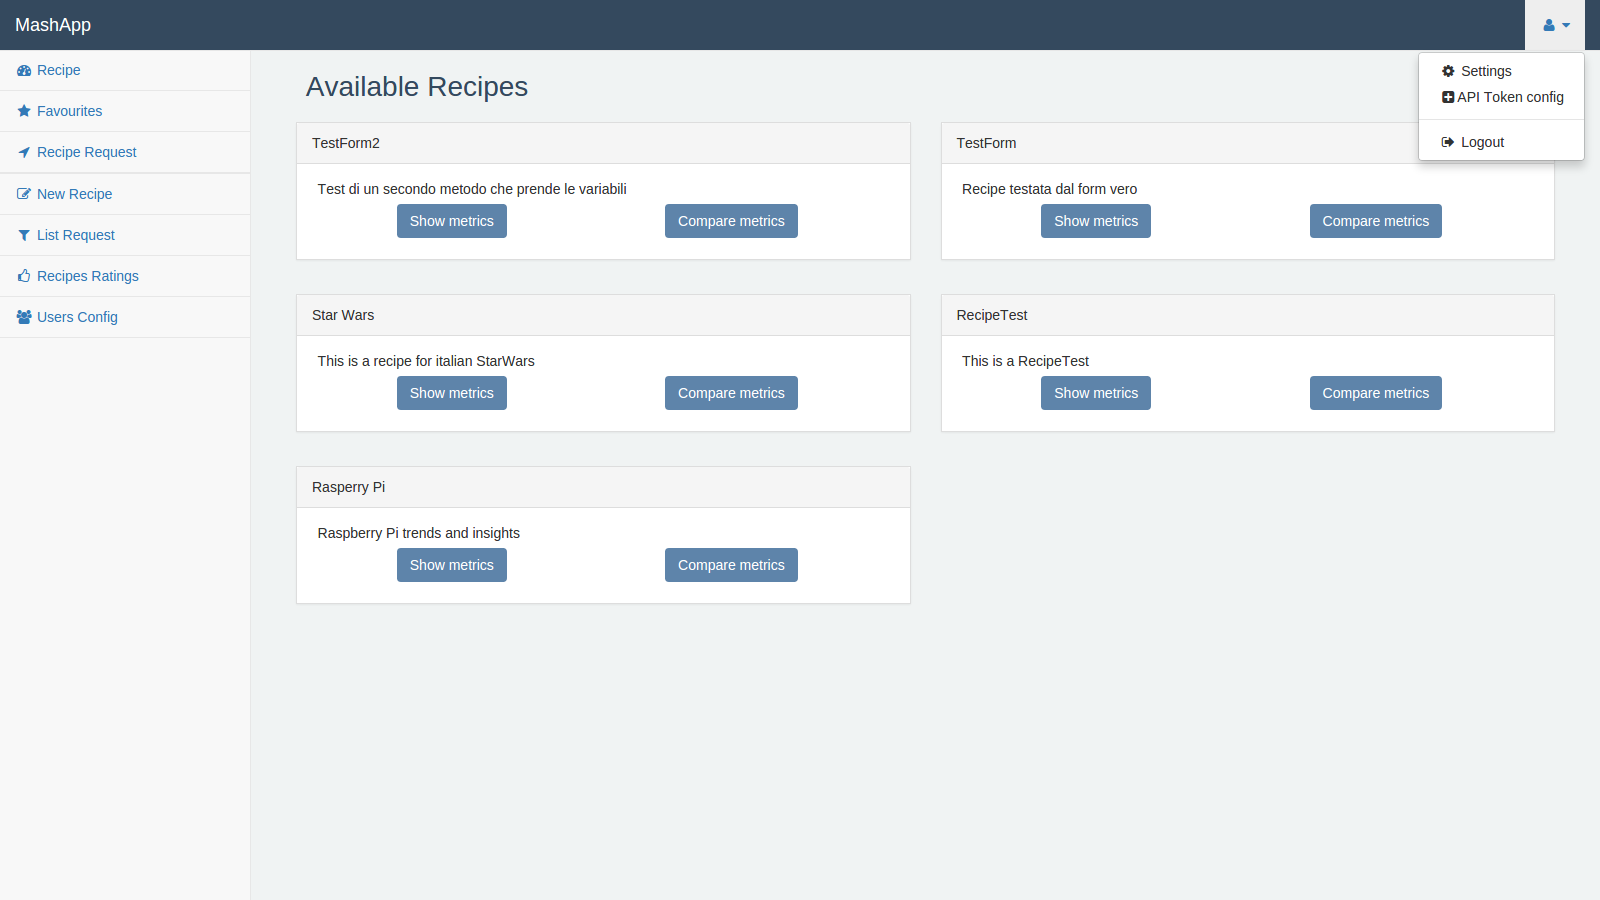
\includegraphics[width=6cm]{images/menu_configurazione_utente.png}}
		\caption{Menu configurazione utente}
		\label{fig:menu_configurazione_utente}
	\end{figure}


	\pagebreak
	\subsection{Settings utente} % (fold)
	\label{sec:settings_utente}
		Cliccando sull'elemento \textbf{settings} (Figura: \ref{fig:menu_configurazione_utente}, rif. 2); nel menù utente si carica la pagina \textbf{General profile settings} (Figura: \ref{fig:configurazione_utente}).
		\begin{figure}[H]
			\centering
			\centerline{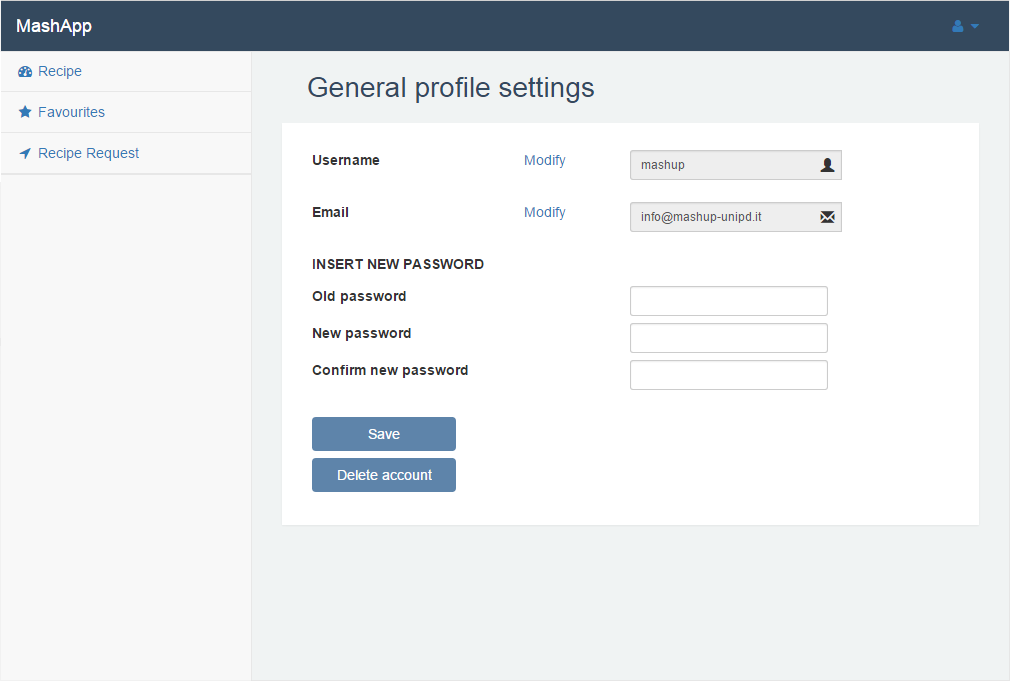
\includegraphics[width=14cm]{images/configurazione_utente.png}}
			\caption{Configurazione utente}
			\label{fig:configurazione_utente}
		\end{figure}
		Dalla pagina di amministrazione si possono effettuare le seguenti operazioni:
		\begin{itemize}
			\item \textbf{modifica username}: per abilitare la modifica è necessario premere sul link a sinistra \textbf{modify} così da sbloccare il riquadro ed editare il campo dati (Figura: \ref{fig:configurazione_utente}, rif. 1);
			\item \textbf{modifica email}: per abilitare la modifica è necessario premere sul link a sinistra \textbf{modify} così da sbloccare il riquadro ed editare il campo dati (Figura: \ref{fig:configurazione_utente}, rif. 2);
			\item \textbf{modifica password}: per cambiare la password è necessario inserire la vecchia password nel primo campo (Figura: \ref{fig:configurazione_utente}, rif. 3) e successivamente la nuova password nei relativi due campi (Figura: \ref{fig:configurazione_utente}, rif. 4 e 5).
		\end{itemize}
		Le modifiche avranno successo solamente quanto verrà premuto il pulsante \textbf{Save} (Figura: \ref{fig:configurazione_utente}, rif. 6).\newline
		Dal pannello di controllo utente è possibile eliminare l'utente corrente premendo sul pulsante \textbf{Delete account} (Figura: \ref{fig:configurazione_utente}, rif. 7). Questo prevede l'eliminazione di tutti i dati utente e il logout dall'applicazione.
	% section Settings utente (end)


	\pagebreak
	\subsection{Configurazione API Token} % (fold)
	\label{sec:settings_utente}
		Cliccando sull'elemento \textbf{API Token config} nel menù utente (Figura: \ref{fig:menu_configurazione_utente}, rif. 3) si carica la pagina \textbf{Token\gloss{} managment} (Figura: \ref{fig:token_config}).
		\begin{figure}[H]
			\centering
			\centerline{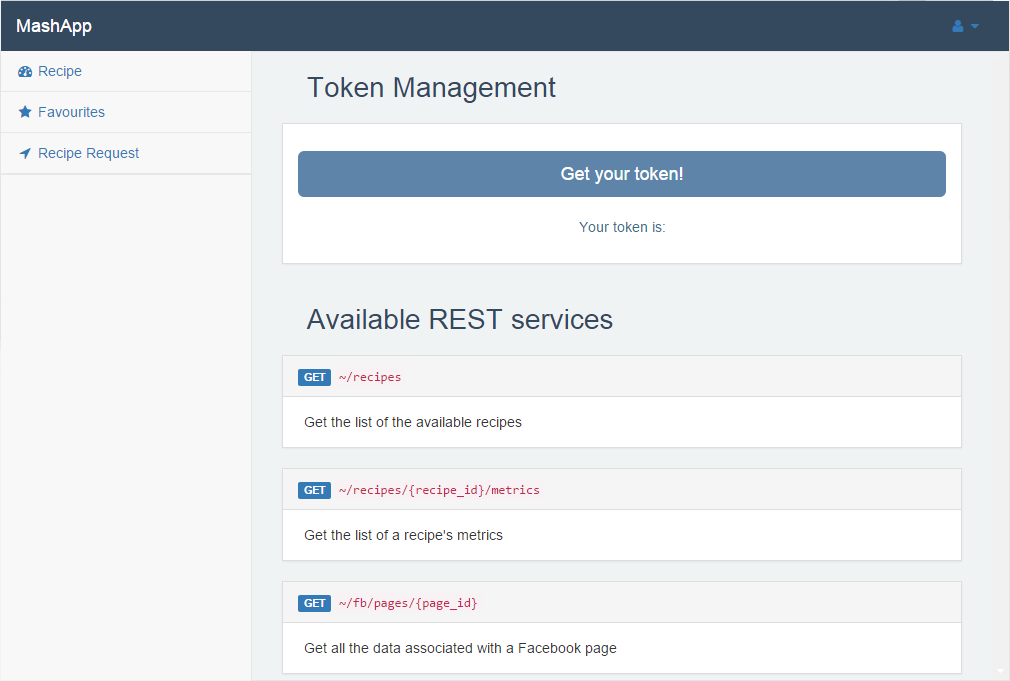
\includegraphics[width=14cm]{images/token_config.png}}
			\caption{Pagina gestione API e token}
			\label{fig:token_config}
		\end{figure}
		\noindent
		Nella seguente pagina (Figura: \ref{fig:token_config}) si possono visualizzare sulla parte inferiore tutte le API\gloss{} che il sistema mette a disposizione (Figura: \ref{fig:token_config}, rif. 2). Tutti i servizi REST\gloss{} offerti dichiarano titolo, metodo e descrizione.\newline
		Per usufruire dei servizi REST\gloss{} è necessario ottenere il \textbf{token}\gloss{} di autenticazione\gloss{} alla piattaforma.\newline 
		É possibile ottenere il token\gloss{} premendo sul pulsante \textbf{Get your token!} (Figura: \ref{fig:token_config}, rif. 1).\newline
		Successivamente sarà possibile visualizzare la stringa contenente il token\gloss{} (Figura: \ref{fig:token_generate}, rif. 1). Da questo punto in poi si potranno utilizzare i servizi REST\gloss{} messi a disposizione dall'applicazione.
		Si può richiedere la rimozione del token premendo sul pulsante \textbf{Delete your token!} (Figura: \ref{fig:token_generate}, rif. 2). All'utente è permesso la rigenerazione del token ogni volta che ne abbia necessità.

		\begin{figure}[H]
			\centering
			\centerline{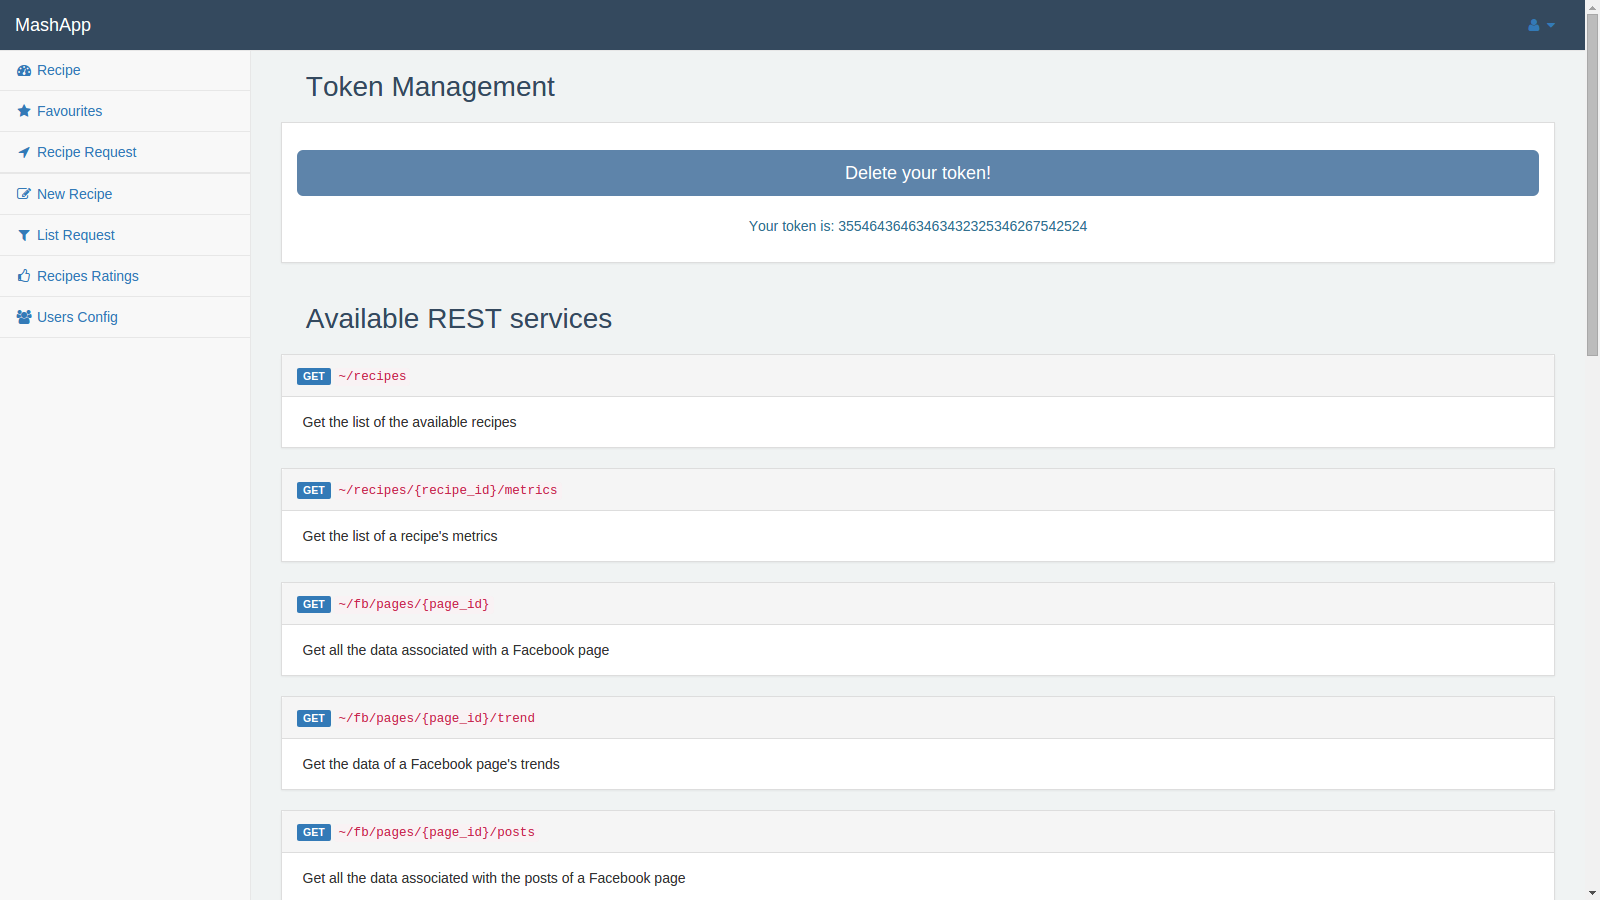
\includegraphics[width=14cm]{images/token_generate.png}}
			\caption{Generazione token utente}
			\label{fig:token_generate}
		\end{figure}
	% section Configurazione API Token (end)


	\subsection{Logout} % (fold)
	\label{sec:logout}
		Cliccando sull'elemento \textbf{Logout}\gloss{} nel menù utente (Figura: \ref{fig:menu_configurazione_utente}, rif. 4) è possibile effettuare la disconnessione dal portale.\newline
		Se il processo avverrà correttamente si caricherà la schermata di autenticazione\gloss{} (Figura: \ref{fig:registrazione_utente_accesso}), sarà così possibile chiudere il browser\gloss{}.		
	% section Logout (end)


% section Configurazione utente (end)